\chapter{Probability}
\section{Discrete}
\begin{definition}[Probability Mass Function]
Given a discrete random variable $X$ taking values in $\mathcal{X}=\{v_1,\hdots, v_m\}$, its probability mass function $P:\mathcal{X}\rightarrow[0,1]$ is defined as:
\begin{center}
	$\displaystyle P(v_i)=\prob{X=v_i}$
\end{center}
And satisfies the following conditions:
\begin{itemize}
	\item $P(x)\geq 0$
	\item $\Sum_{x\in\mathcal{X}}P(x)=1$
\end{itemize}
\end{definition}
So a variable is said to be discrete if it can assume $m$ possible values $\{v_1, \hdots, v_m\}$ which are mutual exclusive and if all probability of the values to happen are non-negative and the sum of probabilities of the events must be 1. \newline
\begin{definition}[Expected Value]
The expected value of a random variable $x$, also known as \textit{mean} or \textit{average}, is:
\begin{center}
	$\displaystyle \E{x}=\mu=\Sum_{x\in\mathcal{X}}xP(x)=\Sum_{i=1}^mv_iP(v_i)$
\end{center}
\end{definition}
The expected value is linear: 
\begin{equation}
	\E{\lambda x+\lambda'y}=\lambda \E{x}+\lambda' \E{y}
	\label{eq:expectedValueLinear}
\end{equation}
\begin{definition}[Variance]
The variance of a random variable is the moment of inertia of its probability mass function:
\begin{center}
	$\displaystyle \Var{x}=\sigma^2=\E{(x-\mu)^2}=\Sum_{x\in\mathcal{X}}(x-\mu)^2P(x)$
\end{center}
\end{definition}
Another important value is the standard deviation $\sigma$ which indicates the typical amount of deviation from the mean.\newline
The followings are properties of mean and variance:
\begin{itemize}
	\item \textbf{Second moment}: it's similar to the expected value:
		\begin{center}
			$\displaystyle \E{x^2}=\Sum_{x\in\mathcal{X}}x^2P(x)$
		\end{center} 
	\item It's possible to write the variance in term via the mean:
		\begin{center}
			$\displaystyle \Var{x}=\E{x^2}-\E{x}^2$
		\end{center}
	\item The variance is \textit{not} always linear, for example when the variable is multiplied by a scalar:
		\begin{equation}
			\displaystyle \Var{\lambda x}=\lambda^2\Var{x}
			\label{eq:varianceNotLinear1}
		\end{equation}
	\item The variance of the sum of two variables corresponds to the sum of the variance \textit{only} if the two variables are not \textit{correlated}:
		\begin{equation}
			\displaystyle \Var{x+y}=\Var{x}+\Var{y}
			\label{eq:varianceNotLinear2}
		\end{equation}
\end{itemize}
%
%
%
\section{Discrete Probability Distribution}
%
%
\subsection{Bernoulli}
This probabilistic distribution is used to model a binary event, that is an event that can only result in success or failure. \newline
The probability $p$ of an event $x$ is the probability of success ($x=1$), while the probability of failure ($x=0$) is $1-p$. The probability mass function is:
\[P(x, p)=
\begin{cases}
	p\quad~\text{if}~x=1\\
	1-p\quad~\text{if}~x=0\\
\end{cases}
\]
A scenarios that can be modelled using this distribution is for example the toss of a coin where head is success and tail is failure (or viceversa).
\begin{theorem}[Estimated Value -- Bernoulli]
\begin{center}
	$\displaystyle \E{x}=p$
\end{center}
\end{theorem}
\begin{proof}
\hspace{1cm}\\
\begin{center}
	$\displaystyle \E{x}=\Sum_{x\in X} xP(x)$ \\
	$\displaystyle \E{x}=\Sum_{x\in \{1,0\}} xP(x)$\\
	$\displaystyle \E{x}=0\times (1-p)+1 \times p=p$
\end{center}
\end{proof}
\begin{theorem}[Variance -- Bernoulli]
\begin{center}
	$\displaystyle \Var{x}=p(1-p)$
\end{center}
\end{theorem} 
\begin{proof}
\hspace{1cm}\\
\begin{center}
\begin{tabular}{rcl}
	$\Var{x}$&=&$\E{(x-\mu )^2}=$\\
			&=&$\Sum_{x\in X}(x-\E{x})^2P(x)=$\\
			&=&$\Sum_{x\in X}(x-p)^2P(x)=$\\
			&=&$(0-p)^2(1-p)+(1-p)^2p=$\\
			&=&$p^2-p^3+(1+p^2-2p)p=$\\
			&=&$p^3-p^3+p^2+p-2p^2$\\
\end{tabular}
\end{center}
\[\Var{x}=p(1-p)\]
\end{proof}
The Bernoulli probability can be expressed also via an analytic function which is often used in if-then-else cases:
\begin{center}
	$\displaystyle p(x,p)=p^x(1-p)^{1-x}$
\end{center}
If $x=1$ then only the first term remains, resulting in $p(x,p)=p$, while if $x=0$, then what remains is: $p(x,p)=1-p$
%
%
\subsection{Binomial}
Bernoulli distribution can be generalized with more than two events: this distribution models the probability of having a certain number of successes in $n$ independent Bernoulli trials.\newline
The parameter of this distribution are $p$ has the probability of a success, and $n$ as the number of trials.\newline
The probability mass function is:
\begin{center}
	$\displaystyle P(x;p,n)=\binom{n}{x}p^x(1-p)^{n-x}$
\end{center}
Which represents the probability of success for $x$ trials and can be seen as the Bernoulli distribution applied to all trials.\newline
An example of event that can be modelled with this distribution is the toss of a coin for $n$ times and trying to guess the probability of having $x$ heads.\newline
Mean and variation are:
\begin{center}
	$\displaystyle \E{x}=np\qquad \Var{x}=np(1-p)$
\end{center}
That is the same as the Bernoulli distribution but multiplied for the $n$ tests.
%
%
\subsection{Joint Probability}
If two random variables are given instead of one, then the model must be different since they may not be independent. 
\begin{definition}[Joint Probability]
Given a pair of discrete random variables $X, Y$ taking values $\mathcal{X}=\{v_1,\hdots,v_m\}, \mathcal{Y}=\{w_1,\hdots,w_n\}$, the joint probability mass function is defined as:
\begin{center}
	$\displaystyle P(v_i,w_i)=\prob{X=v_i, Y=w_j}$
\end{center}
With properties:
\begin{itemize}
	\item $\displaystyle P(x,y)\geq 0$
	\item $\displaystyle \Sum_{x\in\mathcal{X}}\Sum_{y\in\mathcal{Y}}P(x,y)=1$
\end{itemize}
\end{definition}
The characteristics of this function are:
\begin{itemize}
	\item \textit{Expected value}: since there are multiple random variables, then there will be one estimated value for each variable. Mind though that the mean for each variable is not simply the mean for that variable without considering the other variables, but is given by the sum of the value multiplied by the joint probability:
		\begin{center}
			$\displaystyle \mu_x=\E{x}=\Sum_{x\in\mathcal{X}}\Sum_{y\in\mathcal{Y}}xP(x,y)$\\
			\vspace{0.3cm}
			$\displaystyle \mu_y=\E{y}=\Sum_{x\in\mathcal{X}}\Sum_{y\in\mathcal{Y}}yP(x,y)$
		\end{center} 
	\item \textit{Variance}: as for the expected value, there will be one variance for each variable, and they will be computed based on the joint probability:
		\begin{center}
			$\displaystyle \sigma^2_x=\Var{(x-\mu_x)^2}=\Sum_{x\in\mathcal{X}}\Sum_{y\in\mathcal{Y}}(x-\mu_x)^2P(x,y)$\\
					\vspace{0.3cm}
			$\displaystyle \sigma^2_y=\Var{(y-\mu_y)^2}=\Sum_{x\in\mathcal{X}}\Sum_{y\in\mathcal{Y}}(y-\mu_y)^2P(x,y)$
		\end{center}
	\item \textit{Covariance}: this is a statistics of how the random variables change at the change of another variable:
		\begin{center}
			$\displaystyle \sigma_{xy}=\E{(x-\mu_x)(y-\mu_y)}=\Sum_{x\in\mathcal{x}}\Sum_{y\in\mathcal{Y}}(x-\mu_x)(y-\mu_y)=P(x,y)$
		\end{center}
	\item \textit{Correlation coefficient}: it is the normalization of the covariance with respect to the product of the variance:
		\begin{center}
			$\displaystyle \rho=\frac{\sigma_{xy}}{\sigma_x\sigma_y}$
		\end{center}
\end{itemize}
%
\subsubsection{Multinomial Distribution -- One sample}
Models the probability of a certain outcome for an event with $m>2$ possible outcomes\footnote{If $m=2$, then it's simply a Bernoulli distribution.}. \newline
With a multinomial distribution, there are $m$ parameters $p_1, \hdots, p_m$ that indicate the probability of the $j$ outcome to happen. \newline
For example this model represents the tossing of a dice one time, where $m$ is the number of faces of the dice and $p_i$ is the probability of face $i$ to exit. \newline
Since only one sample is considered, then the mass function of this distribution becomes the probability of that event to happen:
\begin{equation}
	P(x_1,\hdots,x_m;p_1\hdots,p_m)=\Prod_{i=1}^mp_i^{x_i}
	\label{eq:MultinomialMassFunction}
\end{equation}
Where if $x_i=1$, then all other outcomes must be 0: $x_j=0, j\neq i$. 
The expected value, the variance are the same as the Bernoulli's while the covariance is:
\begin{center}
	$\displaystyle \E{x_i}=p_i\qquad \Var{x_i}=p_i(1-p_i)\qquad \Cov{x_i, x_j}=-p_ip_j$
\end{center}
%
\subsubsection{Multinomial Distribution -- General}
As for the Bernoulli distribution, also for the multinomial there exists a general version with more samples.\newline
Given $n$ samples of an event with $m$ possible outcomes, the general version models the probability of a certain distribution of outcomes. \newline
For example the following scenario is modelled by a general multinomial distribution: the toss of a coin with $m$ faces, each with $p_i$ probability, $n$ times. \newline
The mass function of this distribution is:
\begin{center}
	$\displaystyle P(x_1,\hdots,x_m;p_1\hdots,p_m)=\cfrac{n!}{\Prod_{i=1}^mx_i!}\Prod_{i=1}^mp_i^{x_i}$
\end{center}
As for the Bernoulli distribution and the bionomial distribution, also in this case the statistics of the general distribution are the same as the one for one sample, just multiplied by $n$. The expected value, variance and covariance are:
\begin{center}
	$\displaystyle \E{x_i}=np_i\qquad \Var{{x_i}=np_i(1-p_i)}\qquad\Cov{x_i,x_j}=-np_ip_j$
\end{center}
%
%
%
\section{Conditional probabilities}
In some cases we want to know the probability of an event to happen given that another event has happened. This is called \textit{conditional probability}:
\begin{definition}[Conditional probability]
The probability of $x$ once $y$ is observed:
\begin{center}
	$\displaystyle P(x\vert y)=\cfrac{P(x,y)}{P(y)}$
\end{center}
\end{definition}
This implies the \textbf{product rule}:
\begin{definition}[Product rule]
\begin{center}
	$\displaystyle P(x,y)=P(x\vert y)P(y)=P(y\vert x)P(x)$
\end{center}
\label{def:ProductRule}
\end{definition}
This rule is useful because it allows to break down a joint probability into a combination of conditional probabilities.\newline 
\begin{definition}[Statistically independence]
	Two variable $X$ and $Y$ are said to be statistically independent if and only if:
\begin{equation}
	P(x,y)=P(x)P(y)
	\label{eq:Independence}
\end{equation}
\label{def:Independence}
\end{definition}
This implies that if two variables $X$ and $Y$ are statistically independent, then:
\begin{center}
	$\displaystyle P(x\vert y)=P(x)\qquad P(y\vert x)=P(y)$
\end{center}
\begin{definition}[Low of Total Probability]
The \textit{marginal distribution} of a variable is obtained from a joint distribution summing over all possible values of the other variable (\textit{sum rule}):
\begin{center}
	$\displaystyle P(x)=\Sum_{y\in\mathcal{Y}}P(x,y)\qquad P(y)=\Sum_{x\in\mathcal{X}}P(x,y)$
\end{center}
\label{def:LawTotalProbability}
\label{def:SumRule}
\end{definition}
This means for example that considering a multinomial variable, it's possible to obtain its probability by removing it from the product and multiplying over the other values.\newline
\begin{definition}[Bayes' Rule]
\begin{center}
	$\displaystyle P(y\vert x)=\cfrac{P(x\vert y)P(y)}{P(x)}$
\end{center}
\label{def:BayesRule}
\end{definition}
Bayes' rule comes from the product rule and allows us to invert the dependency between two probabilities. In particular it allows to invert statistical connections between \textit{effect}(x) and \textit{cause}(y):
\begin{center}
	$\displaystyle \text{posterior}=\cfrac{\text{likelihood}\times\text{prior}}{\text{evidence}}$
\end{center}
Mind that evidence can be obtained using the sum rule from likelihood and prior:
\begin{center}
	$\displaystyle P(x)=\Sum_{y}P(x,y)=\Sum_yP(x\vert y)P(y)$
\end{center}
These rules can be applied to more variables:
\begin{itemize}
	\item \textbf{Sum rule}: $\displaystyle P(y)=\Sum_x\Sum_z P(x,y,z)$
	\item \textbf{Product rule}: apply the first rule more times, for example $P(x,y,z)=P(x\vert y,z)P(y,z)=P(x\vert y,z)P(y\vert z)P(z)=P(x,y,z)=P(x,y\vert z)p(z)$
	\item \textbf{Bayes' rule}: $\displaystyle P(y\vert x,z)=\cfrac{P(x\vert y,z)P(y\vert z)}{P(x\vert z}$
\end{itemize}
Let's compute the probability of $y$ applying these rules:\newline
For the sum rule (aka law of total), we know that:
\begin{center}
	$\displaystyle P(y)=\Sum_x\Sum_z P(x,y,z)$
\end{center}
And for the product rule we know that:
\begin{center}
	$\displaystyle P(x,y,z)=P(y\vert x, z)P(x, z)$
\end{center}
Hence:
\begin{center}
	$\displaystyle P(y)=\Sum_x\Sum_zP(y\vert x, z)P(x, z)$
\end{center}
At last applying Bayes' rule to $P(y\vert x, z)$ we obtain:
\begin{center}
	$\displaystyle P(y)=\Sum_x\Sum_z \cfrac{P(x\vert y,z)P(y\vert z)P(x, z)}{P(x\vert z)}$
\end{center}
%
%
\subsection{Example of style}
Let's start from the following expression and apply the rules:
\begin{center}
	$\displaystyle P(y\vert x,z)$
\end{center}
First of all let's apply Bayes' rule:
\begin{center}
	$\displaystyle P(y\vert x,z)=\cfrac{P(x,z\vert y)P(y)}{P(x,z)}$
\end{center}
Consider the discriminator $P(x,z)$, it's possible to apply the product rule:
\begin{center}
	$\displaystyle P(y\vert x,z)=\cfrac{P(x,z\vert y)P(y)}{P(x\vert z)P(z)}$
\end{center}
Now let's focus on the term $P(x,z\vert y)$. We can imagine it to come from $P(x,z,y)$ to which was applied the product rule: $P(x,z,y)=P(x,z\vert y)P(y)$, but it's also true that $P(x,z,y)=P(x\vert z,y)P(z\vert y)P(y)$, and hence $P(x,z\vert y)=P(x\vert z,y)P(z\vert y)$. It's possible then to rewrite the before as:
\begin{center}
	$\displaystyle P(y\vert x,z)=\cfrac{P(x\vert z,y)P(z\vert y)P(y)}{P(x\vert z)P(z)}$
\end{center}
Now focus on $P(z\vert y)P(y)$, it's obvious that by reversing the product rule, it equals $P(z,y)$, which can be written also as $P(y\vert z)P(z)$ since $P(z,y)=p(y,z)$:
\begin{center}
	$\displaystyle P(y\vert x,z)=\cfrac{P(x\vert z,y)P(y\vert z)P(z)}{P(x\vert z)P(z)}$
\end{center}
At last it's possible to simplify $P(z)$:
\begin{center}
	$\displaystyle P(y\vert x,z)=\cfrac{P(x\vert z,y)P(y\vert z)}{P(x\vert z)}$
\end{center}
%
%
%
\section{Continuos variable}
It's not possible to represent continuous variables with mass function since even if it had a small value, for as small it can be, we are summing it infinite times making it infinite. \newline
Let's consider a continuous variable $X$ and let's consider some intervals: $W=(a<X\leq b),~A=(x\leq a),~B(X\leq b)$. It's possible to notice that $W$ and $A$ are mutually esclusive, hence it's possible to write:
\begin{center}
	$\displaystyle P(B)=P(A)+P(W)\qquad P(W)=P(B)-P(A)$
\end{center}
\begin{definition}[Cumulative Distribution Function]
A function $F(q)$ that models the probability of a continuous variable of having a value less or equal to $q$ is called cumulative distributed function:
\begin{center}
	$\displaystyle F(q)=P(X\leq q)$
\end{center}
\end{definition}
Mind that this is a monotonic function non decreasing: if the interval is enlarged, or it stays the same or it increases.\newline
It's possible to get the probability of intervals by computing the difference between the cumulative distribution functions of the extremities:
\begin{center}
	$\displaystyle P(a<X\leq)=F(b)-F(a)$
\end{center}
\begin{definition}[Probability Density Function]
The derivative of the cumulative distribution function is called probability density function and it represents the probability in a single point:
\begin{center}
	$\displaystyle p(x)=\frac{d}{dx}F(x)$
\end{center}
\end{definition}
The cumulative distribution can also be computed from the density function integrating:
\begin{center}
	$\displaystyle F(q)=P(X\leq q)=\int_{-\infty}^q p(x)dx$
\end{center}
The following are properties of the density function:
\begin{itemize}
	\item $\displaystyle p(x)\geq 0$: which implies that the density probability can also be greater than 1;
	\item $\displaystyle \int_{-\infty}^\infty p(x)dx=1$: even if the density function can be grater than 1, the total integral over the possible values is 1. 
\end{itemize}
Let's consider the following density distribution, the uniform distribution over $[a,b]$:
\begin{center}
	$\displaystyle p(x)=Unif(x;a,b)=\cfrac{1}{b-a}$
\end{center}
For $a=0, b=\myfrac{1}{2}$, then $\forall x\in[0,\myfrac{1}{2}], p(x)=2$. Let's now check the value of the integral: 
\begin{center}
	$F(0<x\leq \myfrac{1}{2})=\displaystyle \int_{-\infty}^{+\infty}p(x)dx=\int_a^bp(x)dx=\int_0^{\frac{1}{2}}2dx=[2x]^{\myfrac{1}{2}}_0=2*\frac{1}{2}-2*0=1$
\end{center}
The expected value of a continuous variable, is computed as the integral of the product of the variable value by its probability:
\begin{center}
	$\displaystyle \E{x}=\mu=\int_{-\infty}^\infty xp(x)dx$
\end{center}
Notice the similarity with the discrete value, only instead of the sum, an integral is used, as can be expected. It should come as no surprise then, the expression for the variance:
\begin{center}
	$\displaystyle \Var{x}=\sigma^2=\int_{-\infty}^\infty(x-\mu)^2p(x)dx$
\end{center}
%
%
\subsection{Gaussian -- Normal}
It is described in terms of $\mu$ and $\sigma^2$ which are its parameters.\newline
It's density function is:
\begin{equation}
	p(x;\mu, \sigma^2)=\frac{1}{\sigma\sqrt{2\pi}}exp-\frac{(x-\mu)^2}{2\sigma^2}
	\label{eq:Gaussian}
\end{equation}
Where the term $\displaystyle \frac{(x-\mu)^2}{2\sigma^2}$ is called standardisation of a normal distribution: $N(\mu,\sigma^2)$, and what it does is basically translate the belle shape and normalize it.\newline
The standard normal distribution is a Gaussian distribution with mean 0 and variance 1. \newline
As it can be expected, the expected value and the variance of the gaussian are $\mu$ and $\sigma^2$ respectively:
\begin{center}
	$\displaystyle \E{x}=\mu\qquad \Var{x}=\sigma^2$
\end{center}

\begin{center}
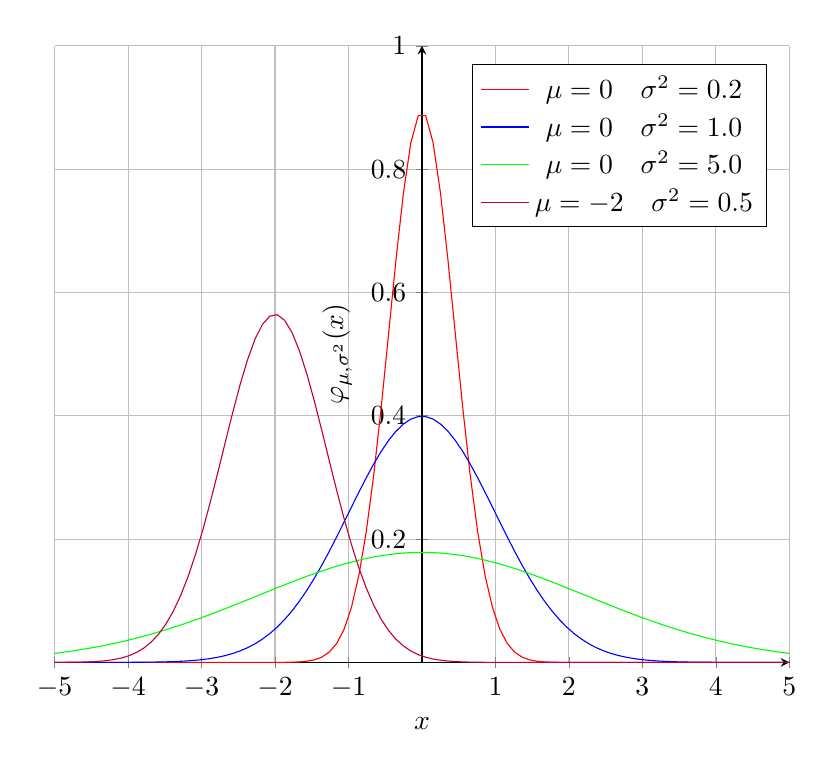
\begin{tikzpicture}
\centering
\begin{axis}[
	width=0.9\linewidth,
	grid=both,
    axis lines = middle,
    xlabel = $x$,
    ylabel = {$\varphi_{\mu,\sigma^2}(x)$},
	xmin=-5, xmax=5,
    ymin=0, ymax=1,
    legend pos=north east,
    ymajorgrids=true,
    legend style={anchor=north east},
    ylabel near ticks,
    xlabel near ticks,
]

\addplot [
    domain=-5:5, 
    samples=100, 
    color=red,
]
{(1/(sqrt(2*3.14)*sqrt(0.2)))*exp(-((x*x)/(2*0.2)))};
\addlegendentry{$\mu=0\quad\sigma^2=0.2$}

\addplot [
    domain=-5:5, 
    samples=100, 
    color=blue,
    ]
{(1/(sqrt(2*3.14)*1))*exp(-((x*x)/(2*1.0)))};
\addlegendentry{$\mu=0\quad\sigma^2=1.0$}

\addplot [
    domain=-5:5, 
    samples=100, 
    color=green,
    ]
{(1/(sqrt(2*3.14)*sqrt(5)))*exp(-((x*x)/(2*5.0)))};
\addlegendentry{$\mu=0\quad\sigma^2=5.0$}

\addplot [
    domain=-5:5, 
    samples=100, 
    color=purple,    
    ] {(1/(sqrt(2*3.14)*sqrt(0.5)))*exp(-((x+2)^2/(2*0.5)))};
\addlegendentry{$\mu=-2\quad\sigma^2=0.5$}
\end{axis}
\end{tikzpicture}
\end{center}
%
%
\subsection{Beta Distribution}
The Beta\footnote{Pronounced /ˈbiːtə/.} distribution is defined inside the interval $[0,1]$. \newline
It is based on parameters $\alpha, \beta$ which let the density function vary as follows:
\begin{equation}
	p(x;\alpha,\beta)=\cfrac{\Gamma(\alpha+\beta)}{\Gamma(\alpha)\Gamma(\beta)}x^{\alpha-1}(1-x)^{\beta-1}
	\label{eq:BetaDensityFunction}
\end{equation}
This distribution can model for example the following scenario: we have a Bernoulli distribution, but no probability distribution for the event to happen is given. Such distribution can be modelled via a Beta distribution, making this a probability of the second order. \newline
Notice that the terms $x^{\alpha-1}, (1-x)^{\beta-1}$ reminds of the binomial one, the beta distribution models the posterior distribution of parameter $p$ of a binomial distribution after observing $\alpha-1$ independent events with probability $p$ and $\beta-1$ events with probability $1-p$.\newline
The expected value and variation are:
\begin{equation}
	\E{x}=\frac{\alpha}{\alpha+\beta}\qquad \Var{x}=\cfrac{\alpha\beta}{(\alpha+\beta)^2(\alpha+\beta+1)}
	\label{eq:BetaStatistics}
\end{equation}
\begin{center}
	\includegraphics[width=0.7\linewidth]{BetaDistribution}
\end{center}
%
%
\subsection{Multivariate Normal Distribution}
This is a normal distribution for $d$-dimensional vectorial data. For this reason the parameters are $\mu$, a vector containing the means, $\Sigma$ a covariance matrix.\newline
It's possible to rewrite the gaussian distribution with the new data by exploiting matrices:
\begin{equation}
	p(\vect{x};\mu,\Sigma)=\cfrac{1}{(2\pi)^{\myfrac{d}{2}}\abs{\Sigma}^{\myfrac{1}{2}}}e^{-\frac{1}{2}(\vect{x}-\vect{\mu})^T\Sigma^{-1}(\vect{x}-\vect{\mu})}
	\label{eq:MultivariateGaussian}
\end{equation}
The term 
\begin{equation}
	\vect{r}^2=(\vect{x}-\vect{\mu})^T\Sigma^{-1}(\vect{x}-\vect{\mu})
	\label{eq:MahalanobisDistance}
\end{equation}
is called Mahalanobis distance and is the generalization of the euclidean distance with respect to the covariance of data. $r^2$ measures the distance from the mean $\vect{\mu}$.\newline
The expected value is actually the expected one: $\E{x}=\mu$, while the variance is actually the covariance parameters: $\Var{x}=\Sigma$.
\begin{center}
	\includegraphics[width=0.8\linewidth]{MultivariateNormalDistribution}
\end{center}

%
%
\subsection{Dirichlet Distribution}
The beta distribution is used to model for example the probability of a binary event. Obviously it can be generalized to the Dirichlet distribution, which is nothing less the continuous version of the multinomial distribution. The Dirichlet distribution allows to model the probability of an event with more than two possible results.\newline
The Dirichlet distribution is defined for $\vect{x}\in[0,1]^m, \Sum_{i=1}^m x_i=1$, that is, given $m$ possible outcomes, $x_1, \hdots, x_m$, the sum of all the outcomes must be 1. \newline
It is parametrized over $\vect{\alpha}=\alpha_1, \hdots, \alpha_m$.\newline
The probability density function is:
\begin{equation}
	p(x_1,\hdots,x_m;\vect{\alpha})=\cfrac{\Gamma(\alpha_0)}{\Prod_{i=1}^m\Gamma(\alpha_i)}\Prod_{i=1}^mx_i^{\alpha_i-1}
	\label{eq:DirichletDensity}
\end{equation}
Where $\alpha_0=\Sum_{j=1}^m\alpha_j$. 
The expected value and variance are the followings:
\begin{equation}
	\E{x_i}=\cfrac{\alpha_i}{\alpha_0}\qquad \Var{x_i}=\cfrac{\alpha_i(\alpha_0-\alpha_i)}{\alpha_0^2(\alpha_0+1)}\qquad\Cov{x_i,x_j}=\cfrac{-\alpha_i\alpha_j}{\alpha_0^2(\alpha_0+1)}
	\label{eq:DirichletStatistics}
\end{equation}
This distribution models the posterior distribution of parameters $\vect{p}$ of a multinomial distribution after observing $\alpha_i-1$ times each mutually exclusive event. 
\begin{center}
	\includegraphics[width=0.8\linewidth]{DirichletDistribution}
\end{center}
%
%
%
\section{Probability Laws}
%
%
\subsection{Expectation and Variance of an Average}
Consider a sample of $X_1,\hdots, X_n$ \textit{independent and identical distributed} (iid) instances drawn from a distribution with mean $\mu$ and variance $\sigma^2$. \newline
Consider the random variable $\overline{X}_n$ measuring the sample average:
\begin{center}
	$\displaystyle \overline{X}_n=\cfrac{X_1+\hdots+X_n}{n}$
\end{center}
Its expectation is computed as:
\begin{center}
	$\displaystyle \E{\overline{X}_n}=\E{\frac{1}{n}(X_1+\hdots+X_n)}$
\end{center}
Now recall that the expected value is linear (Equation \ref{eq:expectedValueLinear}), hence it can be rewritten has:
\begin{center}
	$\displaystyle \E{\overline{X}_n}=\frac{1}{n}(\E{X_1}+\hdots+\E{X_n})$
\end{center}
Since $\E{X_i}=\mu$, then we have:
\begin{center}
	$\displaystyle \E{\overline{X}_n}=\frac{1}{n}(\mu+\hdots+\mu)=\frac{1}{n}*n\mu=\mu$
\end{center}
That is the expectation of an average is the true mean of the distribution. \newline
Now let's consider the variance which though is not linear with respect to scalars (Equation~\ref{eq:varianceNotLinear}), while it behaves linear when summing variances (Equation~\ref{eq:varianceNotLinear2}). It's possible to write the variance of $\overline{X}_n$ as:
\begin{center}
	$\displaystyle \Var{\overline{X}_n}=\frac{1}{n^2}(\Var{X_1}+\hdots+\Var{X_n})=\frac{\sigma^2}{n}$
\end{center}
From this is possible to notice that the variance of the average decreases with the number of observation: the more examples are taken into consideration, the more likely estimating the correct average is. 
%
%
\subsection{Chebyshev's Inequality}
Consider a random variable $X$ with mean $\mu$ and variance $\sigma^2$. The Chebyshev's inequality states that for all $a>0$:
\begin{center}
	$\displaystyle \prob{\abs{X-\mu}\geq a}\leq\frac{\sigma^2}{a^2}$
\end{center}
Replacing $a$ with $k\sigma, k>0$ we obtain:
\begin{center}
	$\displaystyle \prob{\abs{X-\mu}\geq k\sigma}\leq\frac{1}{k^2}$
\end{center}
Chebyshev's inequality shows that most of the probability mass of a random variable stays within few standard deviations from its mean. 
%
%
\section{The Law of Large Numbers}
Let's suppose to have some phenomenon to model and the distribution was not observed in its entirety, but only $n$ events, for example we register only if rains for some days. Let's suppose also that the events are \textit{identically distributed} since they come from the same phenomenon and that they are also independent which implies that the outcome of an event does not affect other events. \newline
Our goal is to evaluate the average and the variance observing the data at our disposal. \newline
Consider a sample of $X_1, \hdots, X_n$ iid instances drawn from a distribution with mean $\mu$ and variance $\sigma^2$. \newline
We have already shown in the previous sections that the expected value of iid samples of mean $\mu$ is actually $\mu$, now it's possible to show through the Chebyshev's inequality that the probability that the sample-mean drifts away from the actual mean of a little value $\\epsilon$ decreases at the increasing of the number of samples. This implies that the accuracy of an empirical statistic increases with the number of samples.
\begin{center}
	$\displaystyle \prob{\abs{\overline{X}_n-\E{\overline{X}_n}}\geq\epsilon}\leq\frac{\sigma^2}{n\epsilon^2}$\\
	\vspace{0.3cm}
	$\displaystyle \lim_{n\rightarrow\infty} \prob{\abs{\overline{X}_n-\mu}\geq \epsilon}=0$
\end{center}
%
%
%
\subsection{Central Limit Theorem}
\begin{definition}[Central Limit Theorem]
The sum of a sufficiently large sample of iid random measurement is approximately normally distributed.
\end{definition}
This means that if we have a number $n$ of samples sufficiently large, with mean $\mu$ and variance $\sigma^2$, we don't need to know the form of their distribution, because they can be modelled through a normal gaussian. \newline
Questo significa che se abbiamo molti dati, se non conosciamo la distribuzione dei dati, allora la possiamo considerare questa distribuzione come una normale. \newline
%
%
%
\section{Information theory}
%
%
\subsection{Entropy}
Consider a set of symbols $\mathcal{V}=\{v_1,\hdots,v_n\}$ with mutually exclusive probabilities $P(v_i)$. \newline
The goal is to design a binary code for each symbol minimizing the average length of messages. In 1949 Shannon and Weaver proved that the optimal code assigns to each symbol $v_i$ a number of bits equal to:
\begin{center}
	$\displaystyle -\log{P(v_i)}$
\end{center}
\begin{definition}[Entropy]
The entropy of a set of symbols is the \textbf{expected value} length of a message encoding a symbol assuming such optimal coding:
\begin{center}
	$\displaystyle H[\mathcal{V}]=\E{-\log{P(v)}}=-\Sum_{i=1}^nP(v_i)\log{P(v_i)}$
\end{center}
\end{definition}
If all symbols have the same probability, then the entropy is maximized, while if the symbols have very much different probabilities, then the entropy becomes 0. \newline
%
%
\subsection{Cross entropy}
\begin{definition}[Cross Entropy]
Given two distributions $P$ and $Q$ over a variable $X$, the cross entropy between $P$ and $Q$ measures the expected number of bits needed to code a symbol sampled from $P$ using $Q$ instead:
\begin{center}
	$\displaystyle H(P;Q)=\text{E}_P[-\log{Q(v)}]=-\Sum_{i=1}^nP(v_i)\log{Q(v_i)}$
\end{center}
\end{definition}
This is often used as a loss function for binary classification, with $P$ (empirical) true distribution and $Q$ (empirical) predicted distribution. 
%
%
\subsection{Relative Entropy}
\begin{definition}[Relative Entropy]
Given two distribution $P, Q$ over a variable $X$, the relative entropy (or \textit{Kullback-Leibler divergence)} measures the expected length difference when coding instances samples from $P$ using $Q$ instead:
\begin{center}
	$\displaystyle D_{KL}(p\Vert q)=\Sum_{i=1}^nP(v_i)\log{\frac{P(v_i)}{Q(v_i)}}$
\end{center}
\end{definition}
This can be derived as follows:
\begin{center}
	\begin{tabular}{rcl}
		$D_{KL}(p\Vert Q)$&=&$H(P;Q)-H(P)$\\
		&=&$\text{E}_P[-\log{Q(v)}]-\E{-\log{P(v)}}$\\
		&=&$-\Sum_{i=1}^nP(v_i)\log{Q(v_i)}+\Sum_{i=1}^nP(v_i)\log{P(v_i)}$\\
		&=&$\Sum_{i=1}^n\left[P(v_i)\log{P(v_i)}-P(v_i)\log{Q(v_i)}\right]$\\
		&=&$\Sum_{i=1}^nP(v_i)\left(\log{P(v_i)}-\log{Q(v_i)}\right)$\\
		&=&$\Sum_{i=1}^nP(v_i)\log{\frac{P(v_i)}{Q(v_i)}}$
	\end{tabular}
\end{center}
%
%
\subsection{Conditional entropy}
\begin{definition}[Conditional Entropy]
Given two variables $V,W$ with possibly different distributions $P$, the conditional entropy is the entropy remaining for variable $W$ once $V$ is known:
\begin{center}
	\begin{tabular}{rcl}
		$H(W\vert V)$&=&$\Sum_vP(v)H(W\vert V=v)$\\
		&=&$-\Sum_{v}P(v)\Sum_wP(w\vert v)\log{P(w\vert v)}$
	\end{tabular}
\end{center}
\end{definition}
This says that, the more we know about $V$, the more is the entropy of $W$, and viceversa.
\subsection{Mutual Information -- Information Gain}
\begin{definition}[Information Gain]
Given two variables $V,W$ with (possibly different) distributions $P$, the mutual information, or information gain, is the reduction in entropy for $W$ once $V$ is known:
\begin{center}
	\begin{tabular}{rcl}
		$I(W; V)$&=&$H(W)-H(W\vert V)$\\
		&=&$-\Sum_{w}p(w)\log{p(w)}+\Sum_vP(v)\Sum_wP(w\vert v)\log{P(w\vert v)}$
	\end{tabular}
\end{center}
\end{definition}
The information gain is the reduction of entropy on $W$ once $V$ is known. This can be used, for example, when deciding which attribute is best to select when building a decision tree, where $V$ is the attribute and $W$ is the label.